\section{Data Analysis}
\begin{figure}
    \begin{center}
        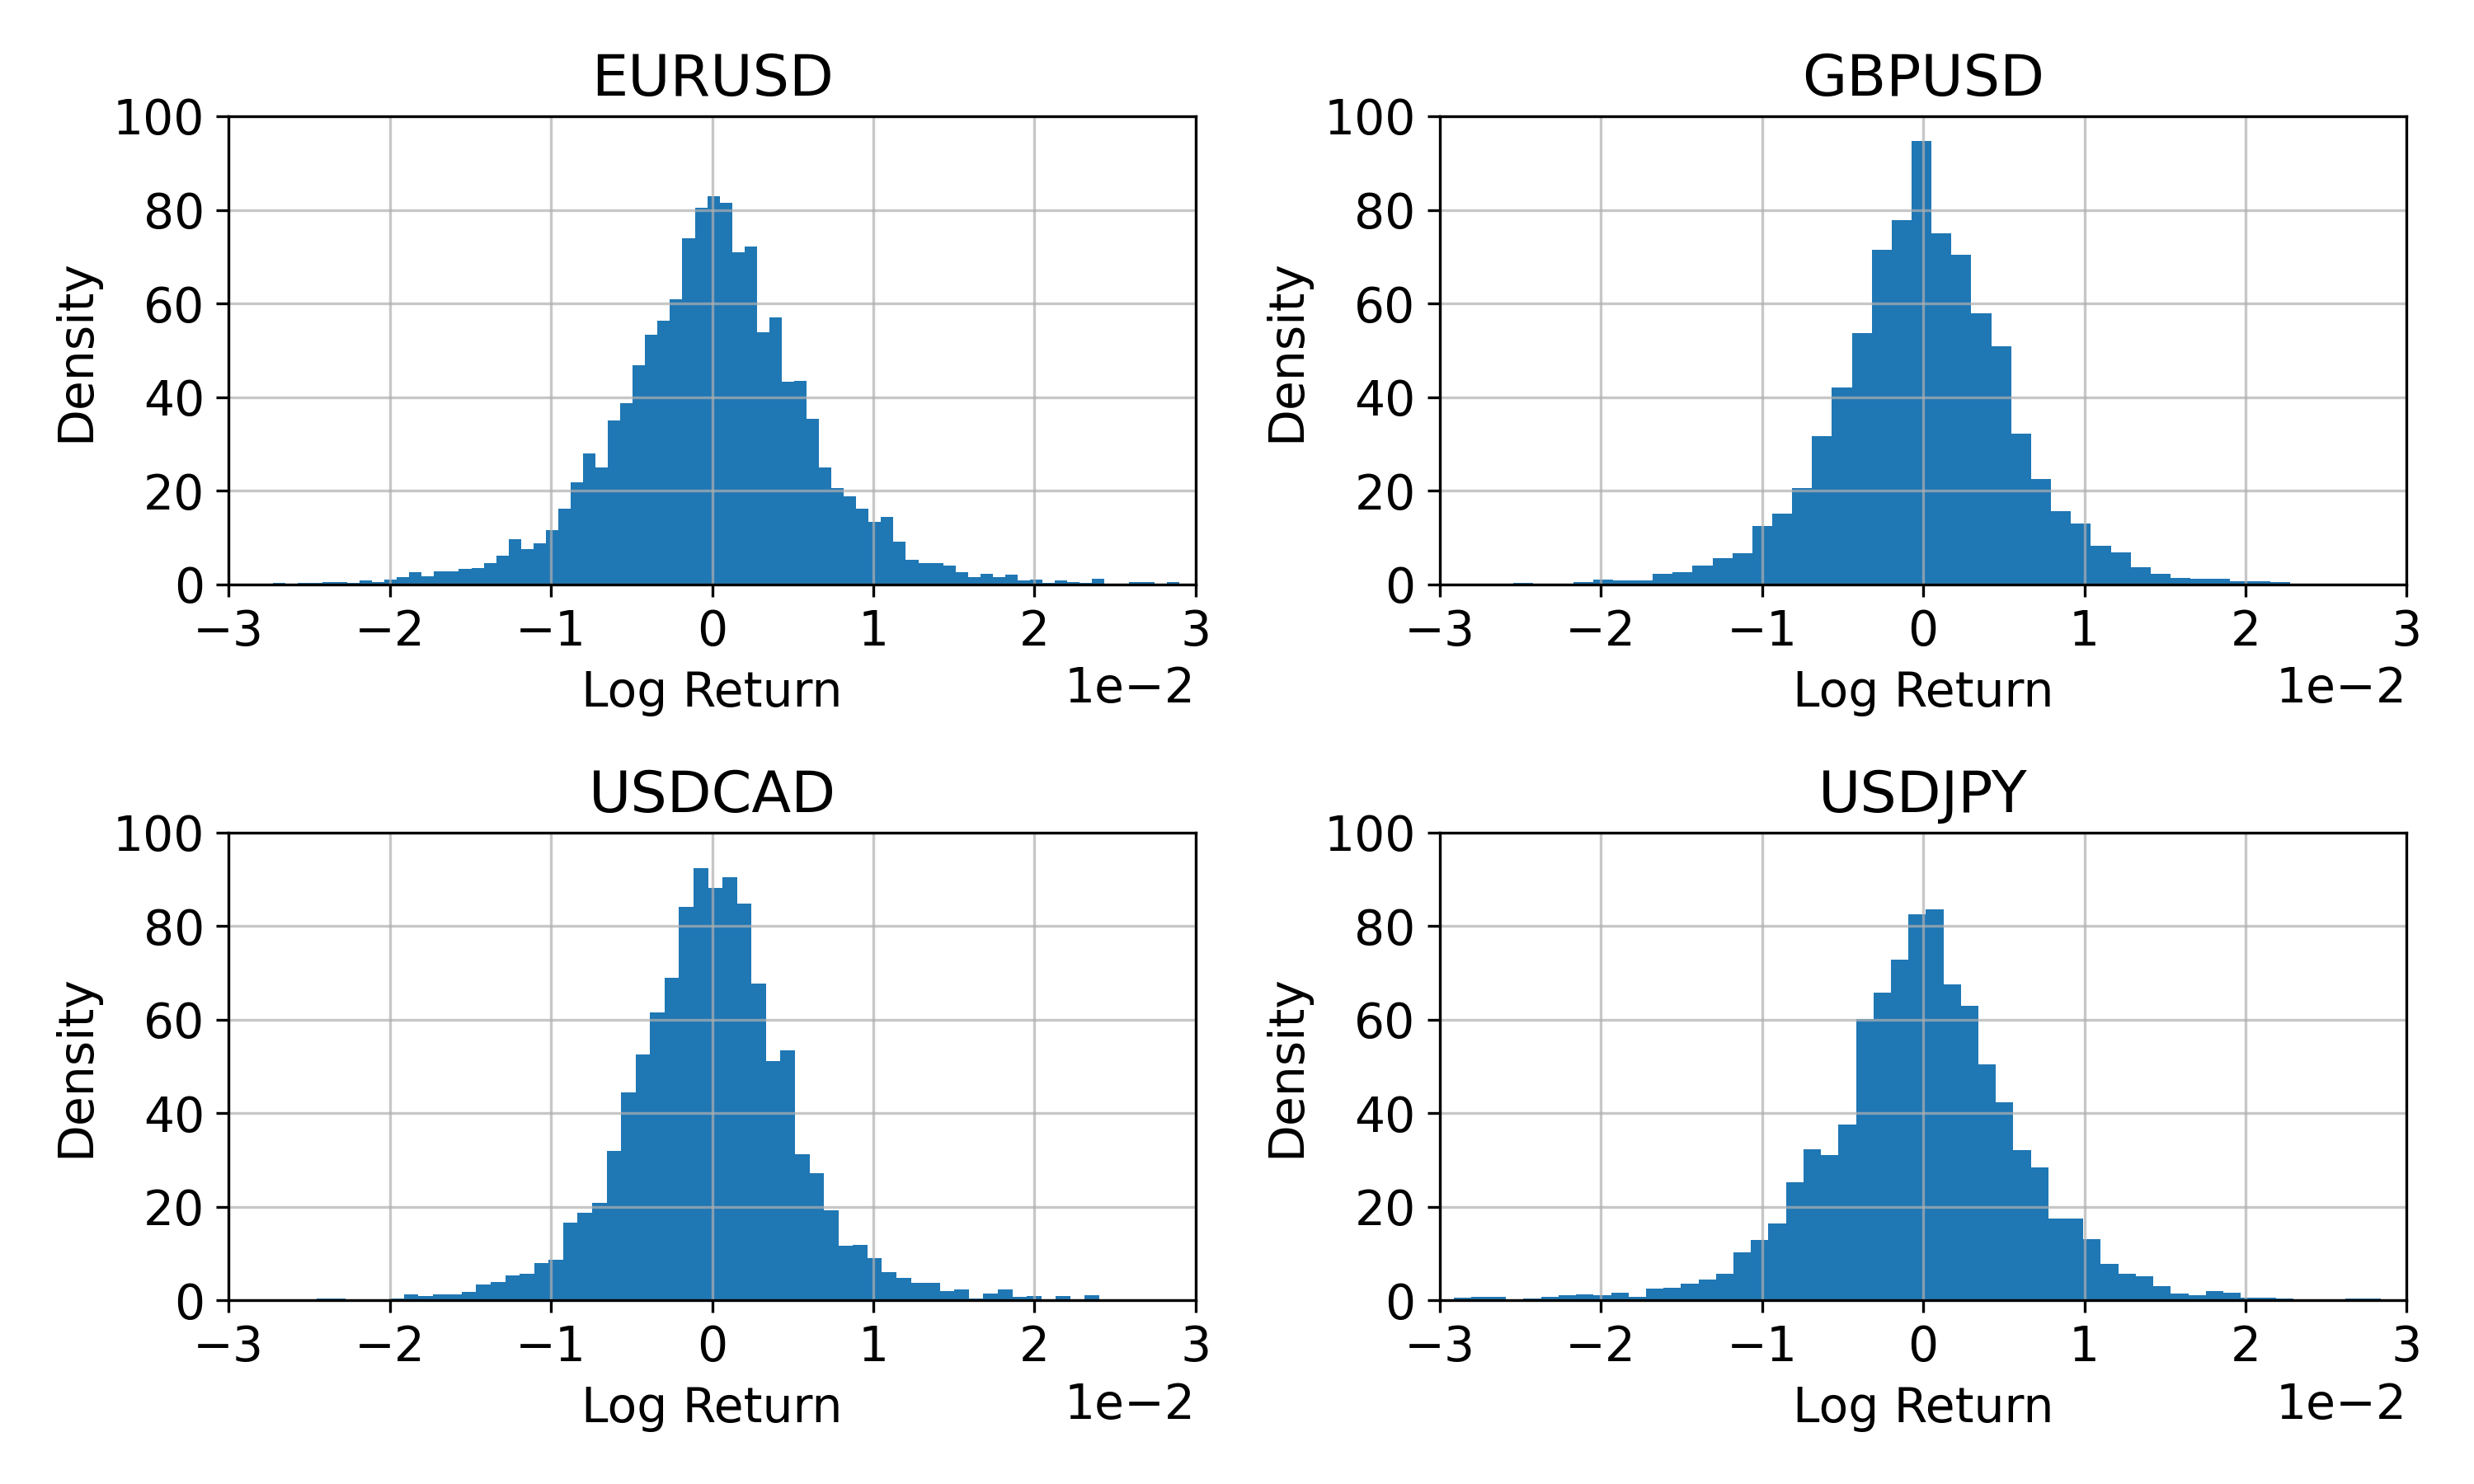
\includegraphics[width=1\linewidth]{data_analysis/histograms.png}
    \end{center}
    \caption{Histograms of the log returns for major currency pairs from 1999-01-01 through 2019-12-31.}
    \label{fig:histograms_raw}
\end{figure}

\begin{figure}
    \begin{center}
        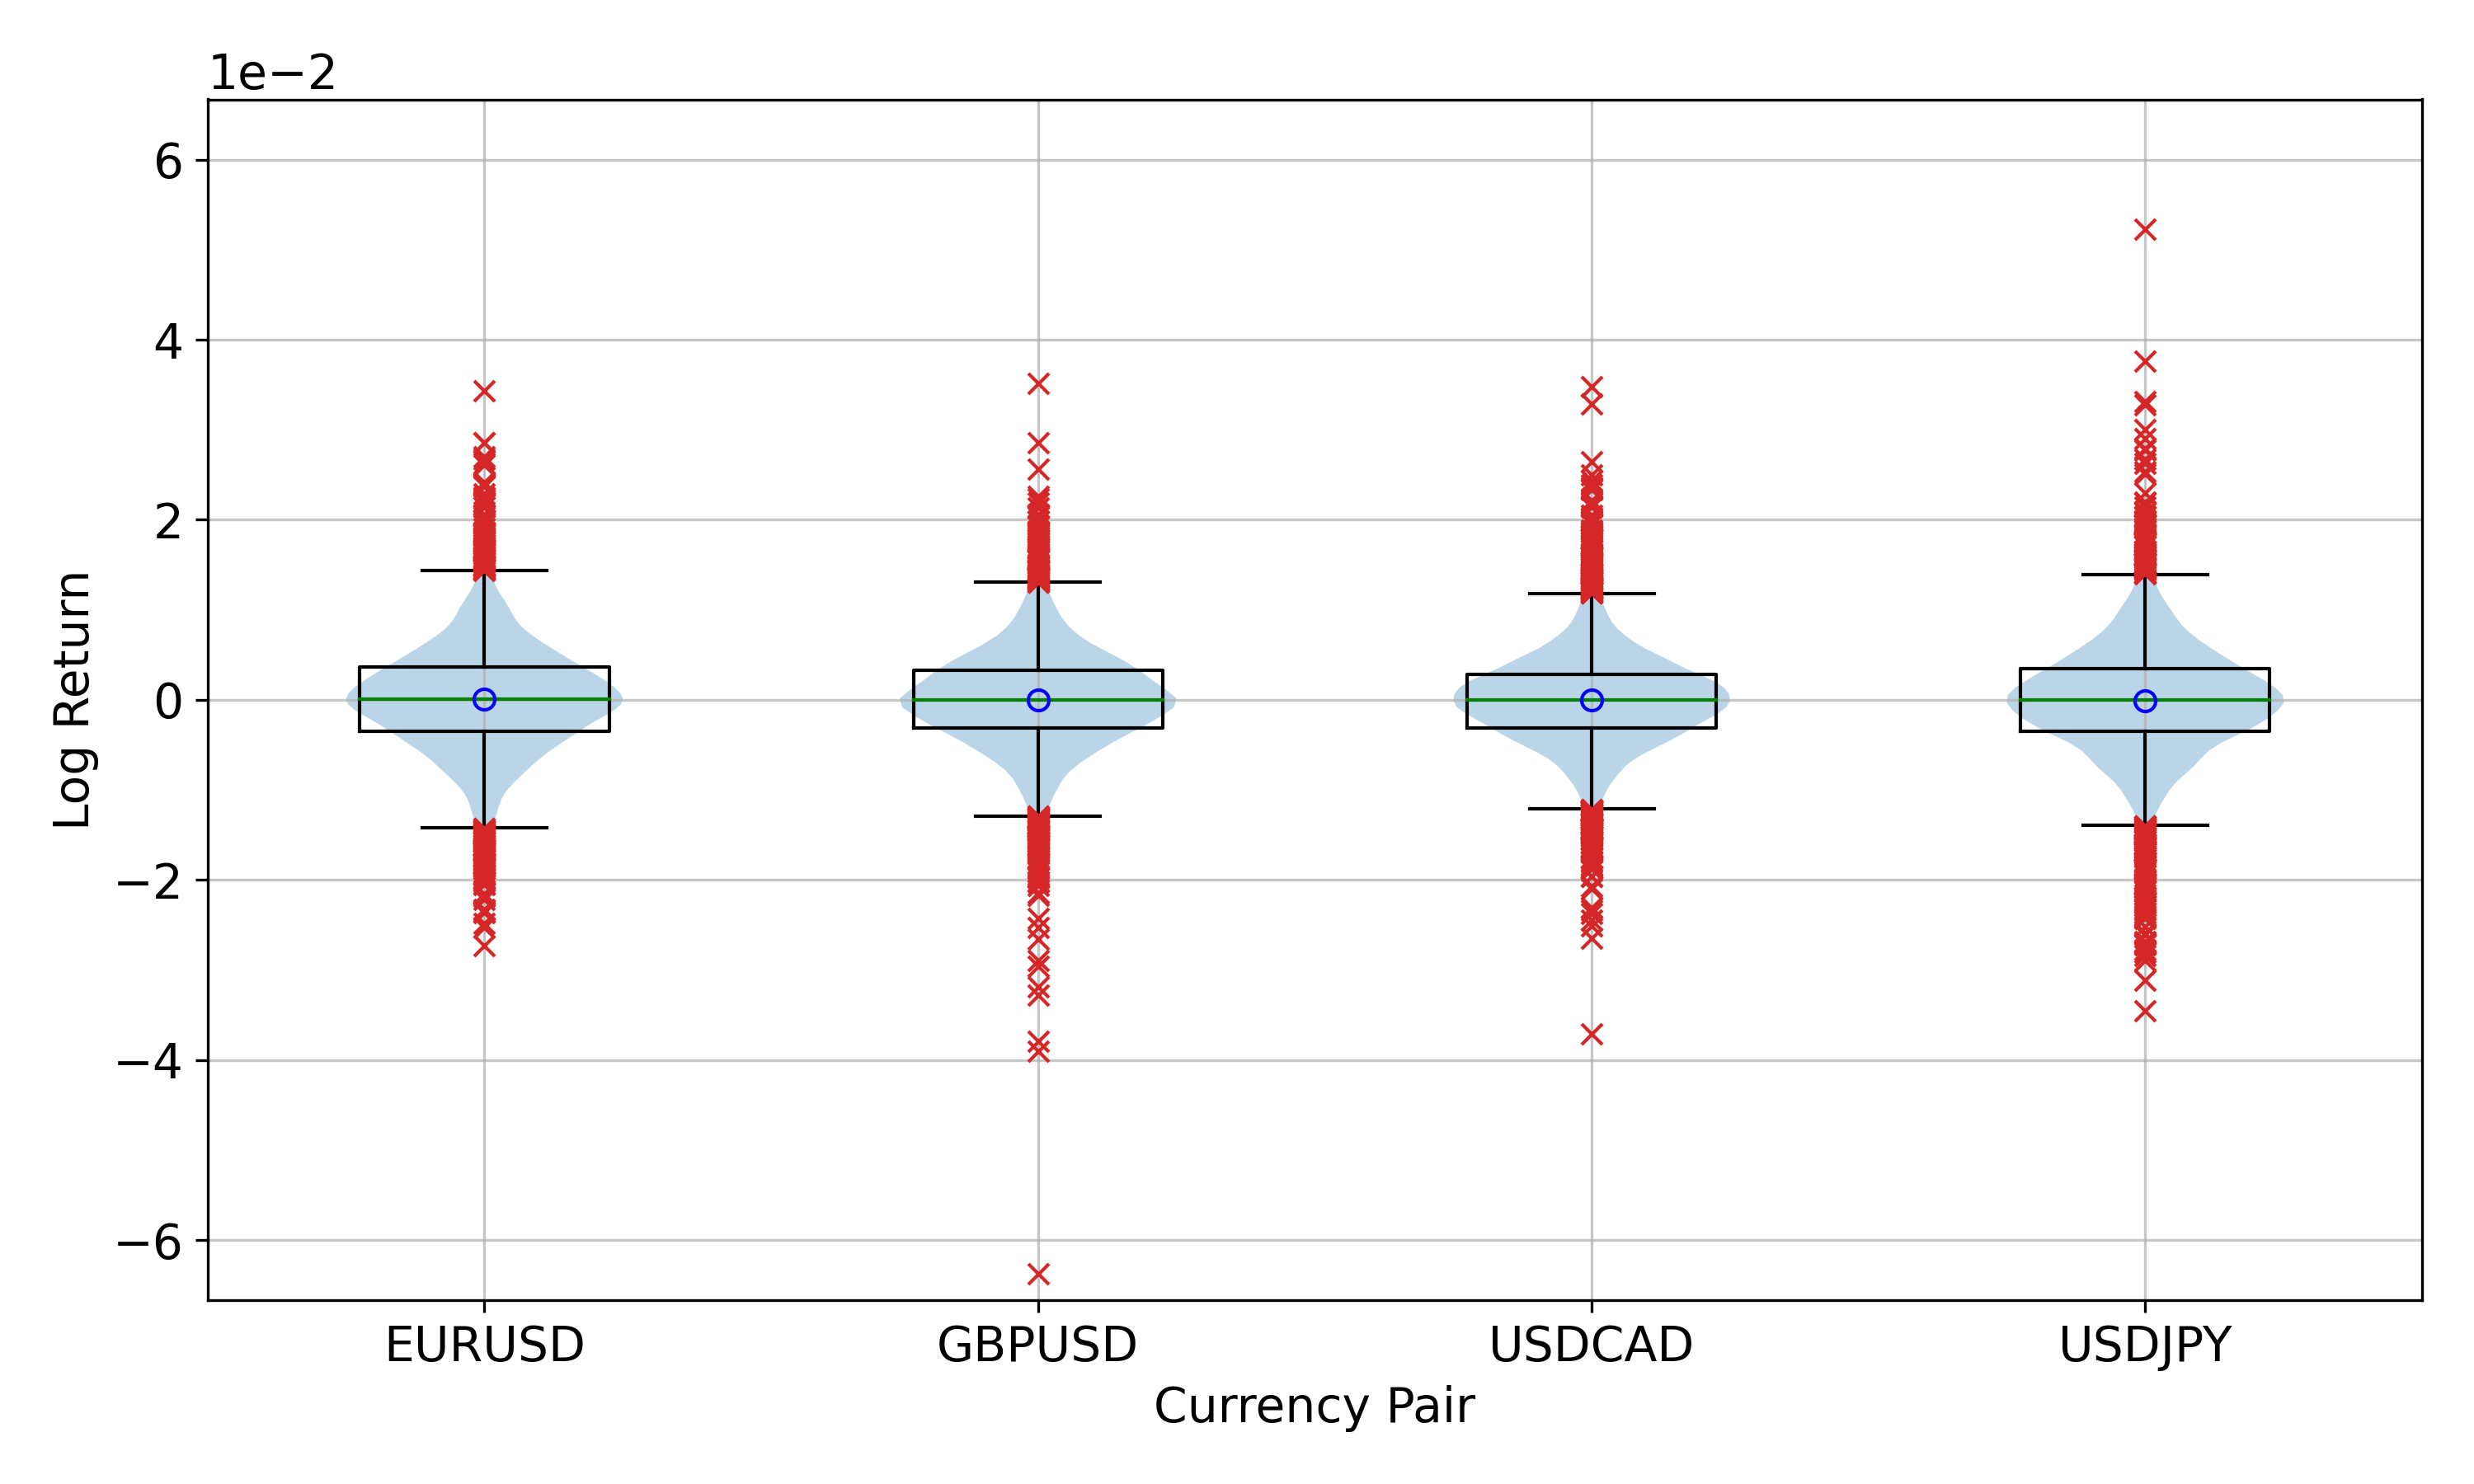
\includegraphics[width=1\linewidth]{data_analysis/violin.png}
    \end{center}
    \caption{Violin/box plot of the log returns for major currency pairs from 1999-01-01 through 2019-12-31.}
    \label{fig:violin_raw}
\end{figure}

\section{Data Preprocessing}
\todo{Algorithm for binarization}

\todo{Algorithm for transformation}

\begin{figure}
    \begin{center}
        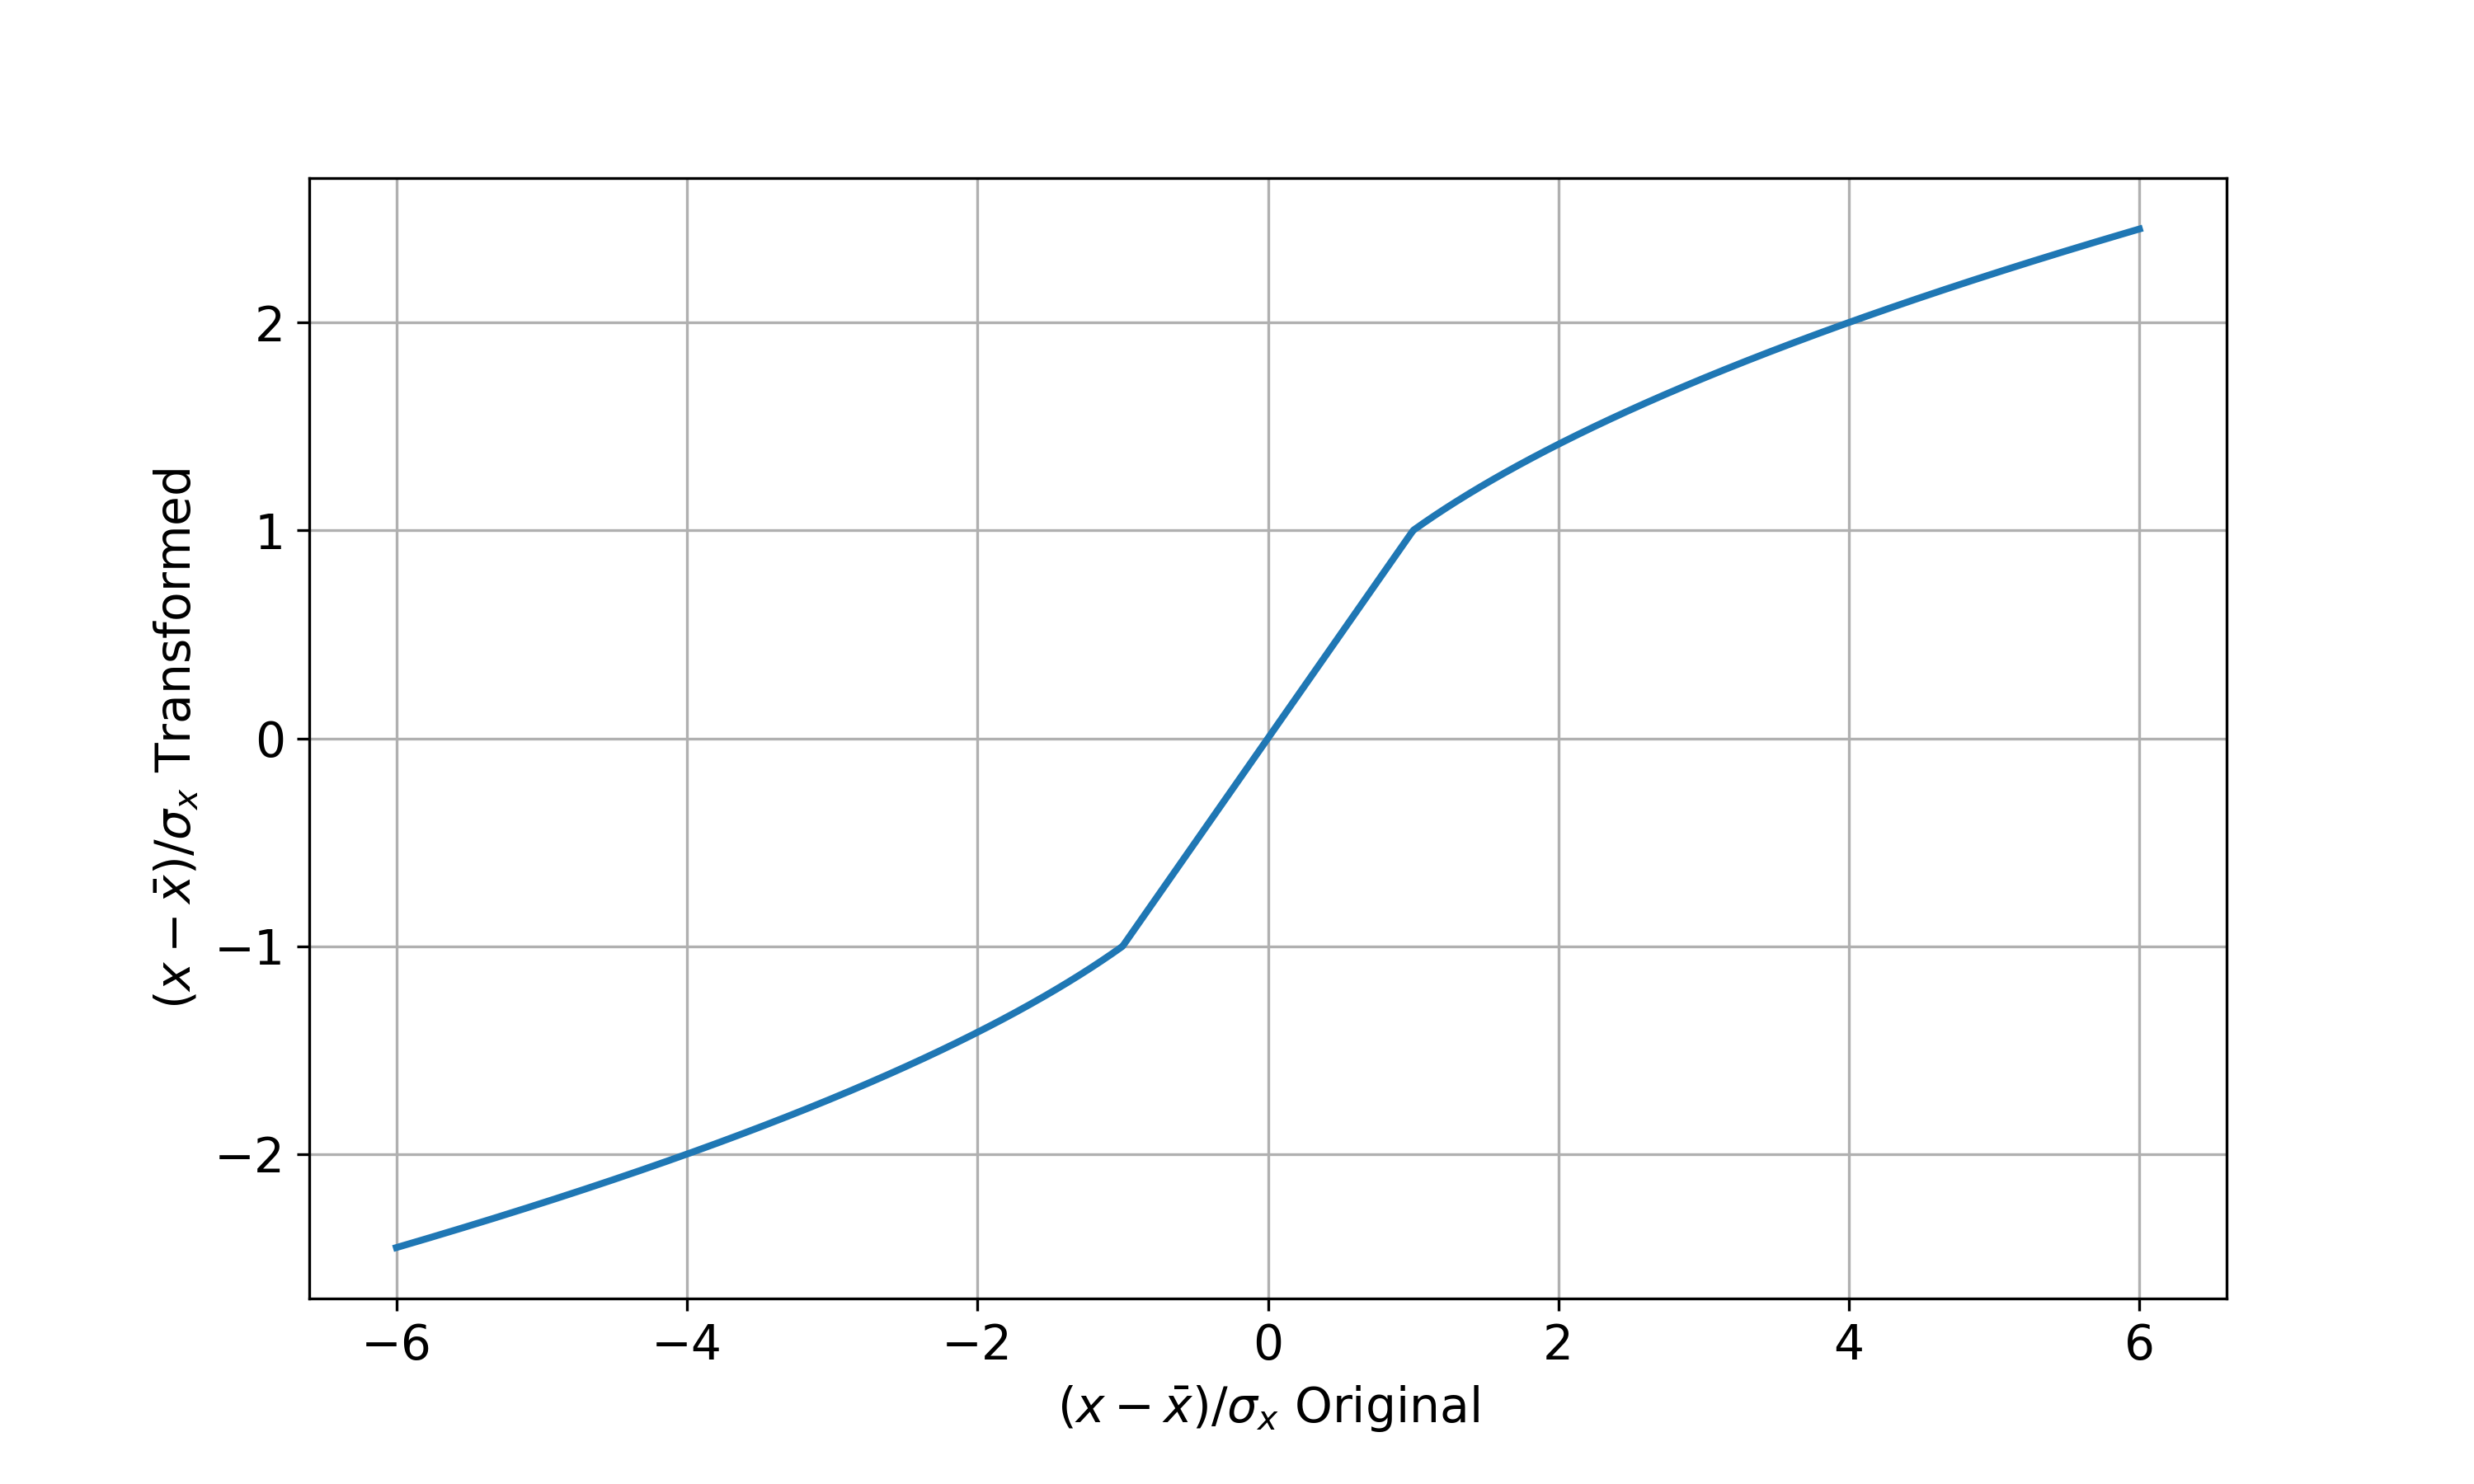
\includegraphics[width=1\linewidth]{data_analysis/data_transformation.png}
    \end{center}
    \caption{Transformation function applied to the data before training, for the purpose of reducing large "gaps" in the binarized data by scaling outliers above one standard deviation by taking the square root of the standardized value.}
    \label{fig:data_transformation}
\end{figure}

\begin{figure}
    \begin{center}
        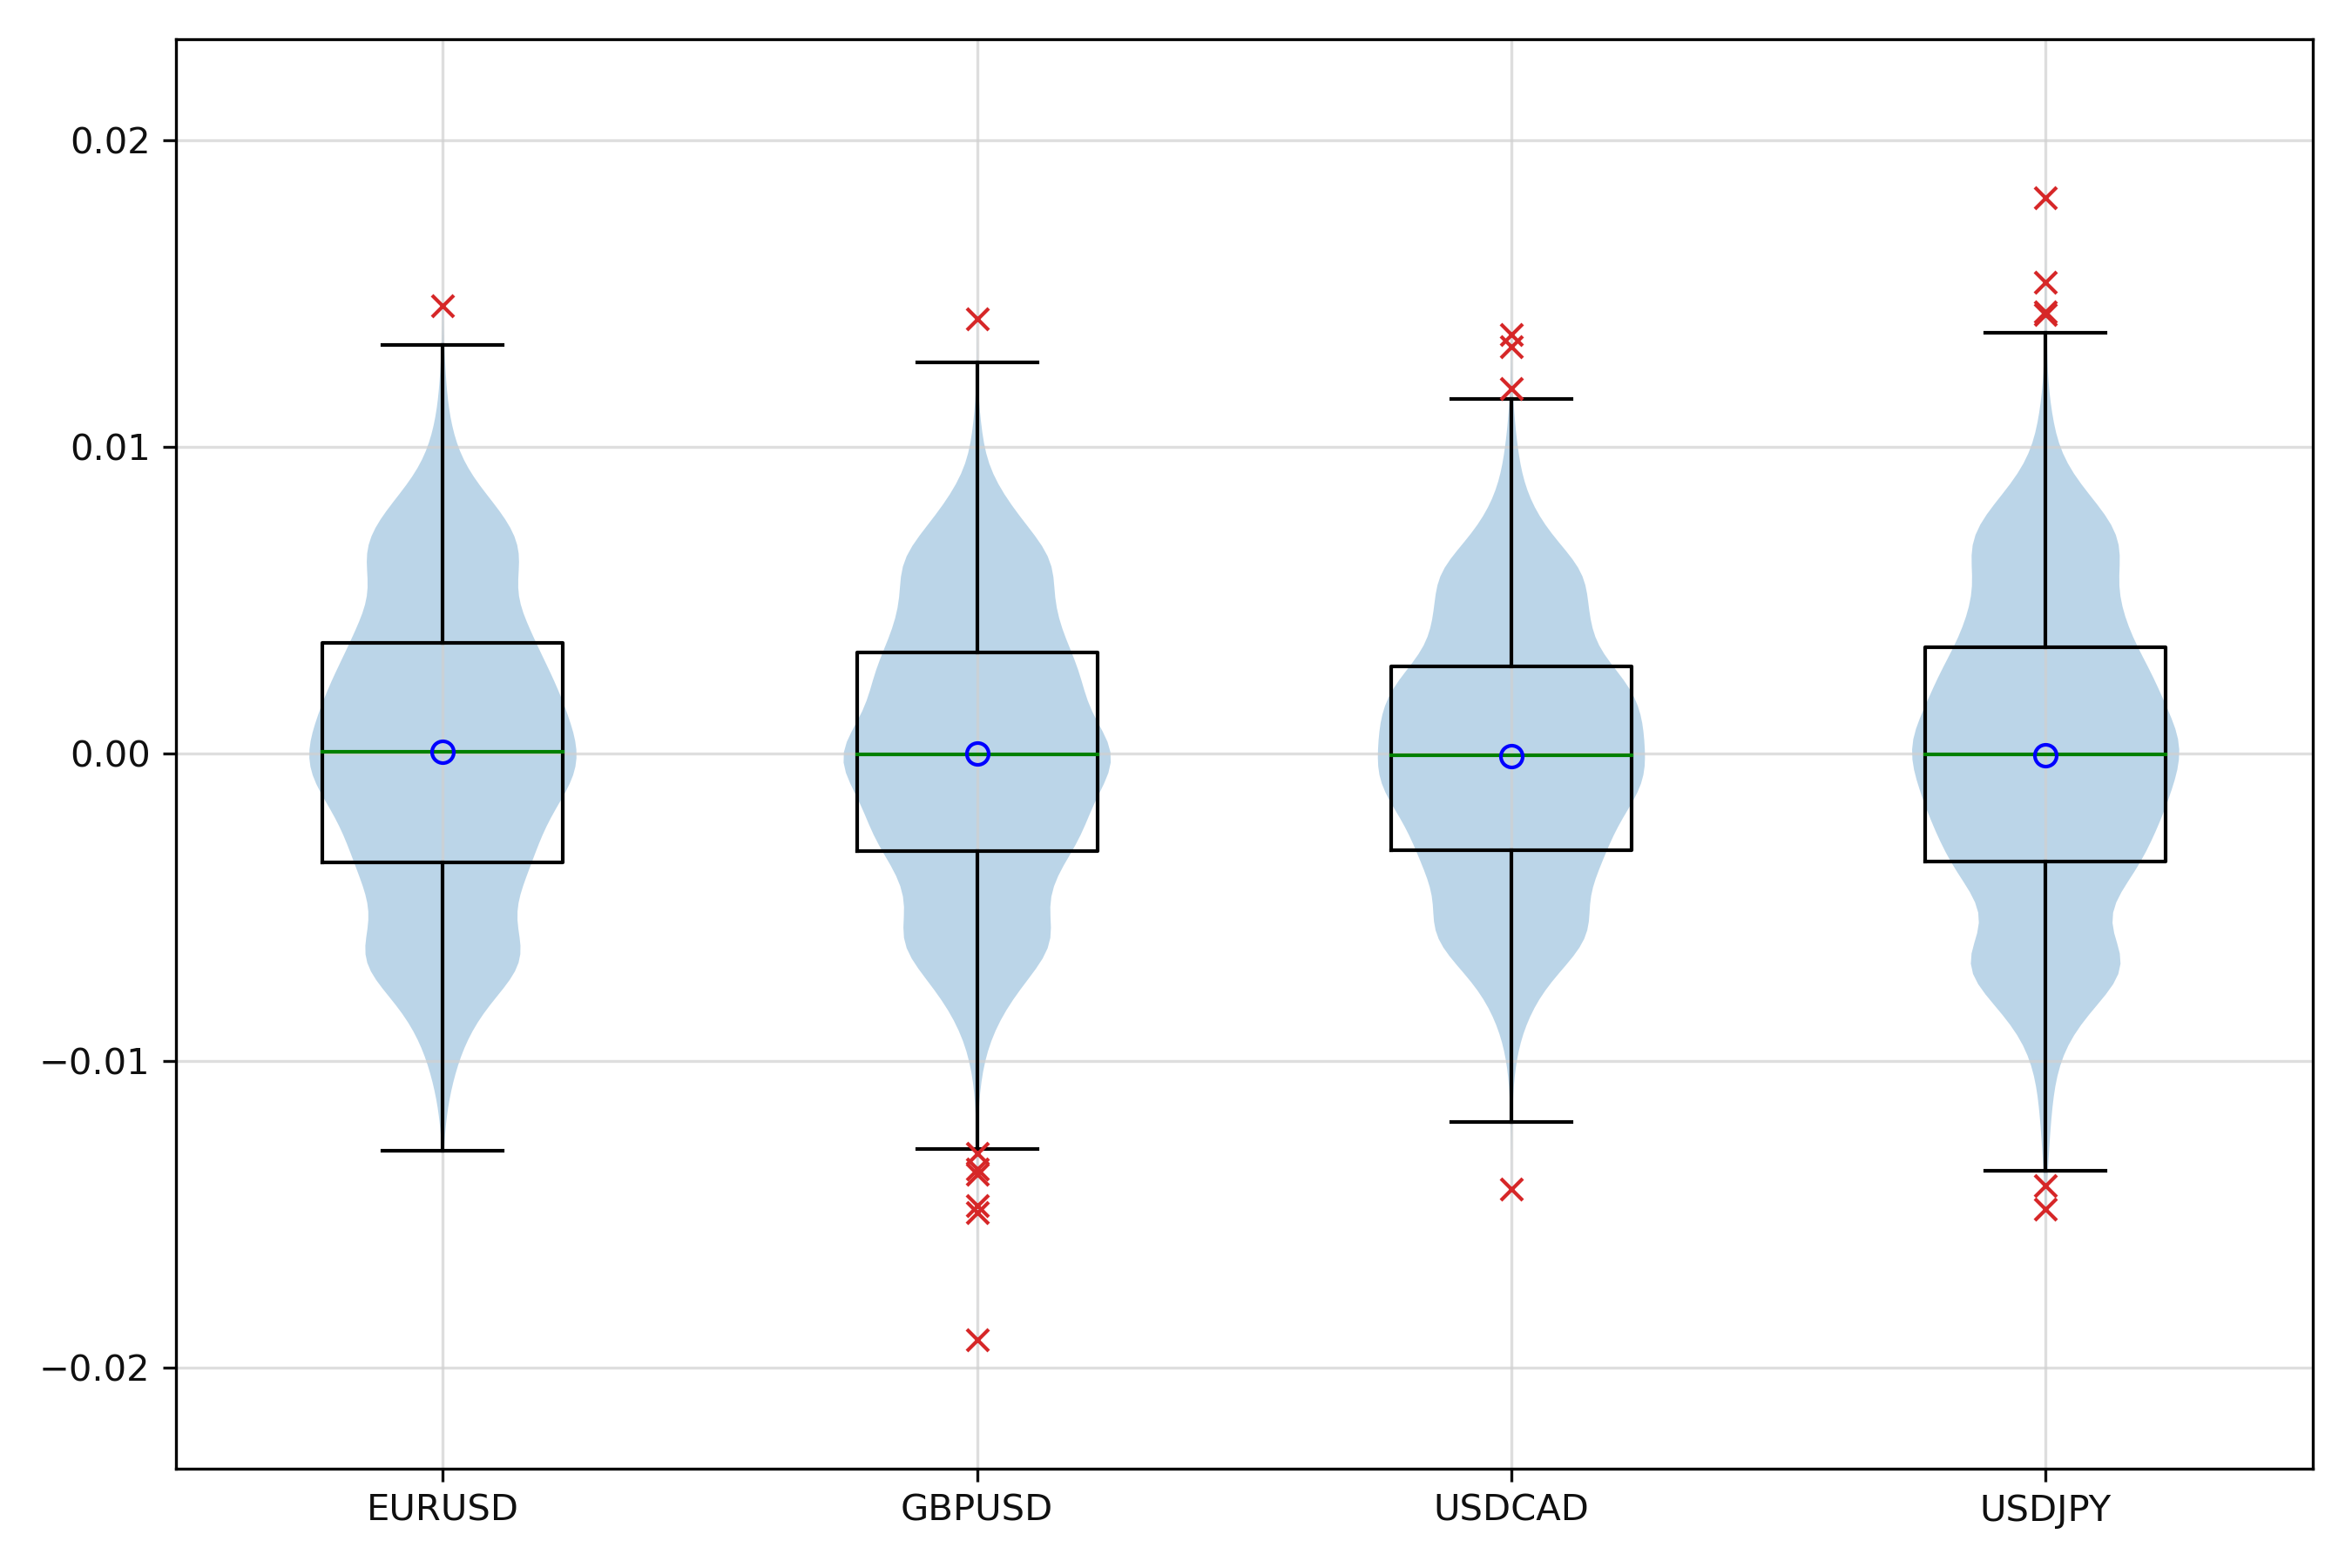
\includegraphics[width=1\linewidth]{data_analysis/violin_transformed.png}
    \end{center}
    \caption{Violin/box plot of the log returns for major currency pairs from 1999-01-01 through 2019-12-31.}
    \label{fig:violin_transformed}
\end{figure}

\begin{figure}
    \begin{center}
        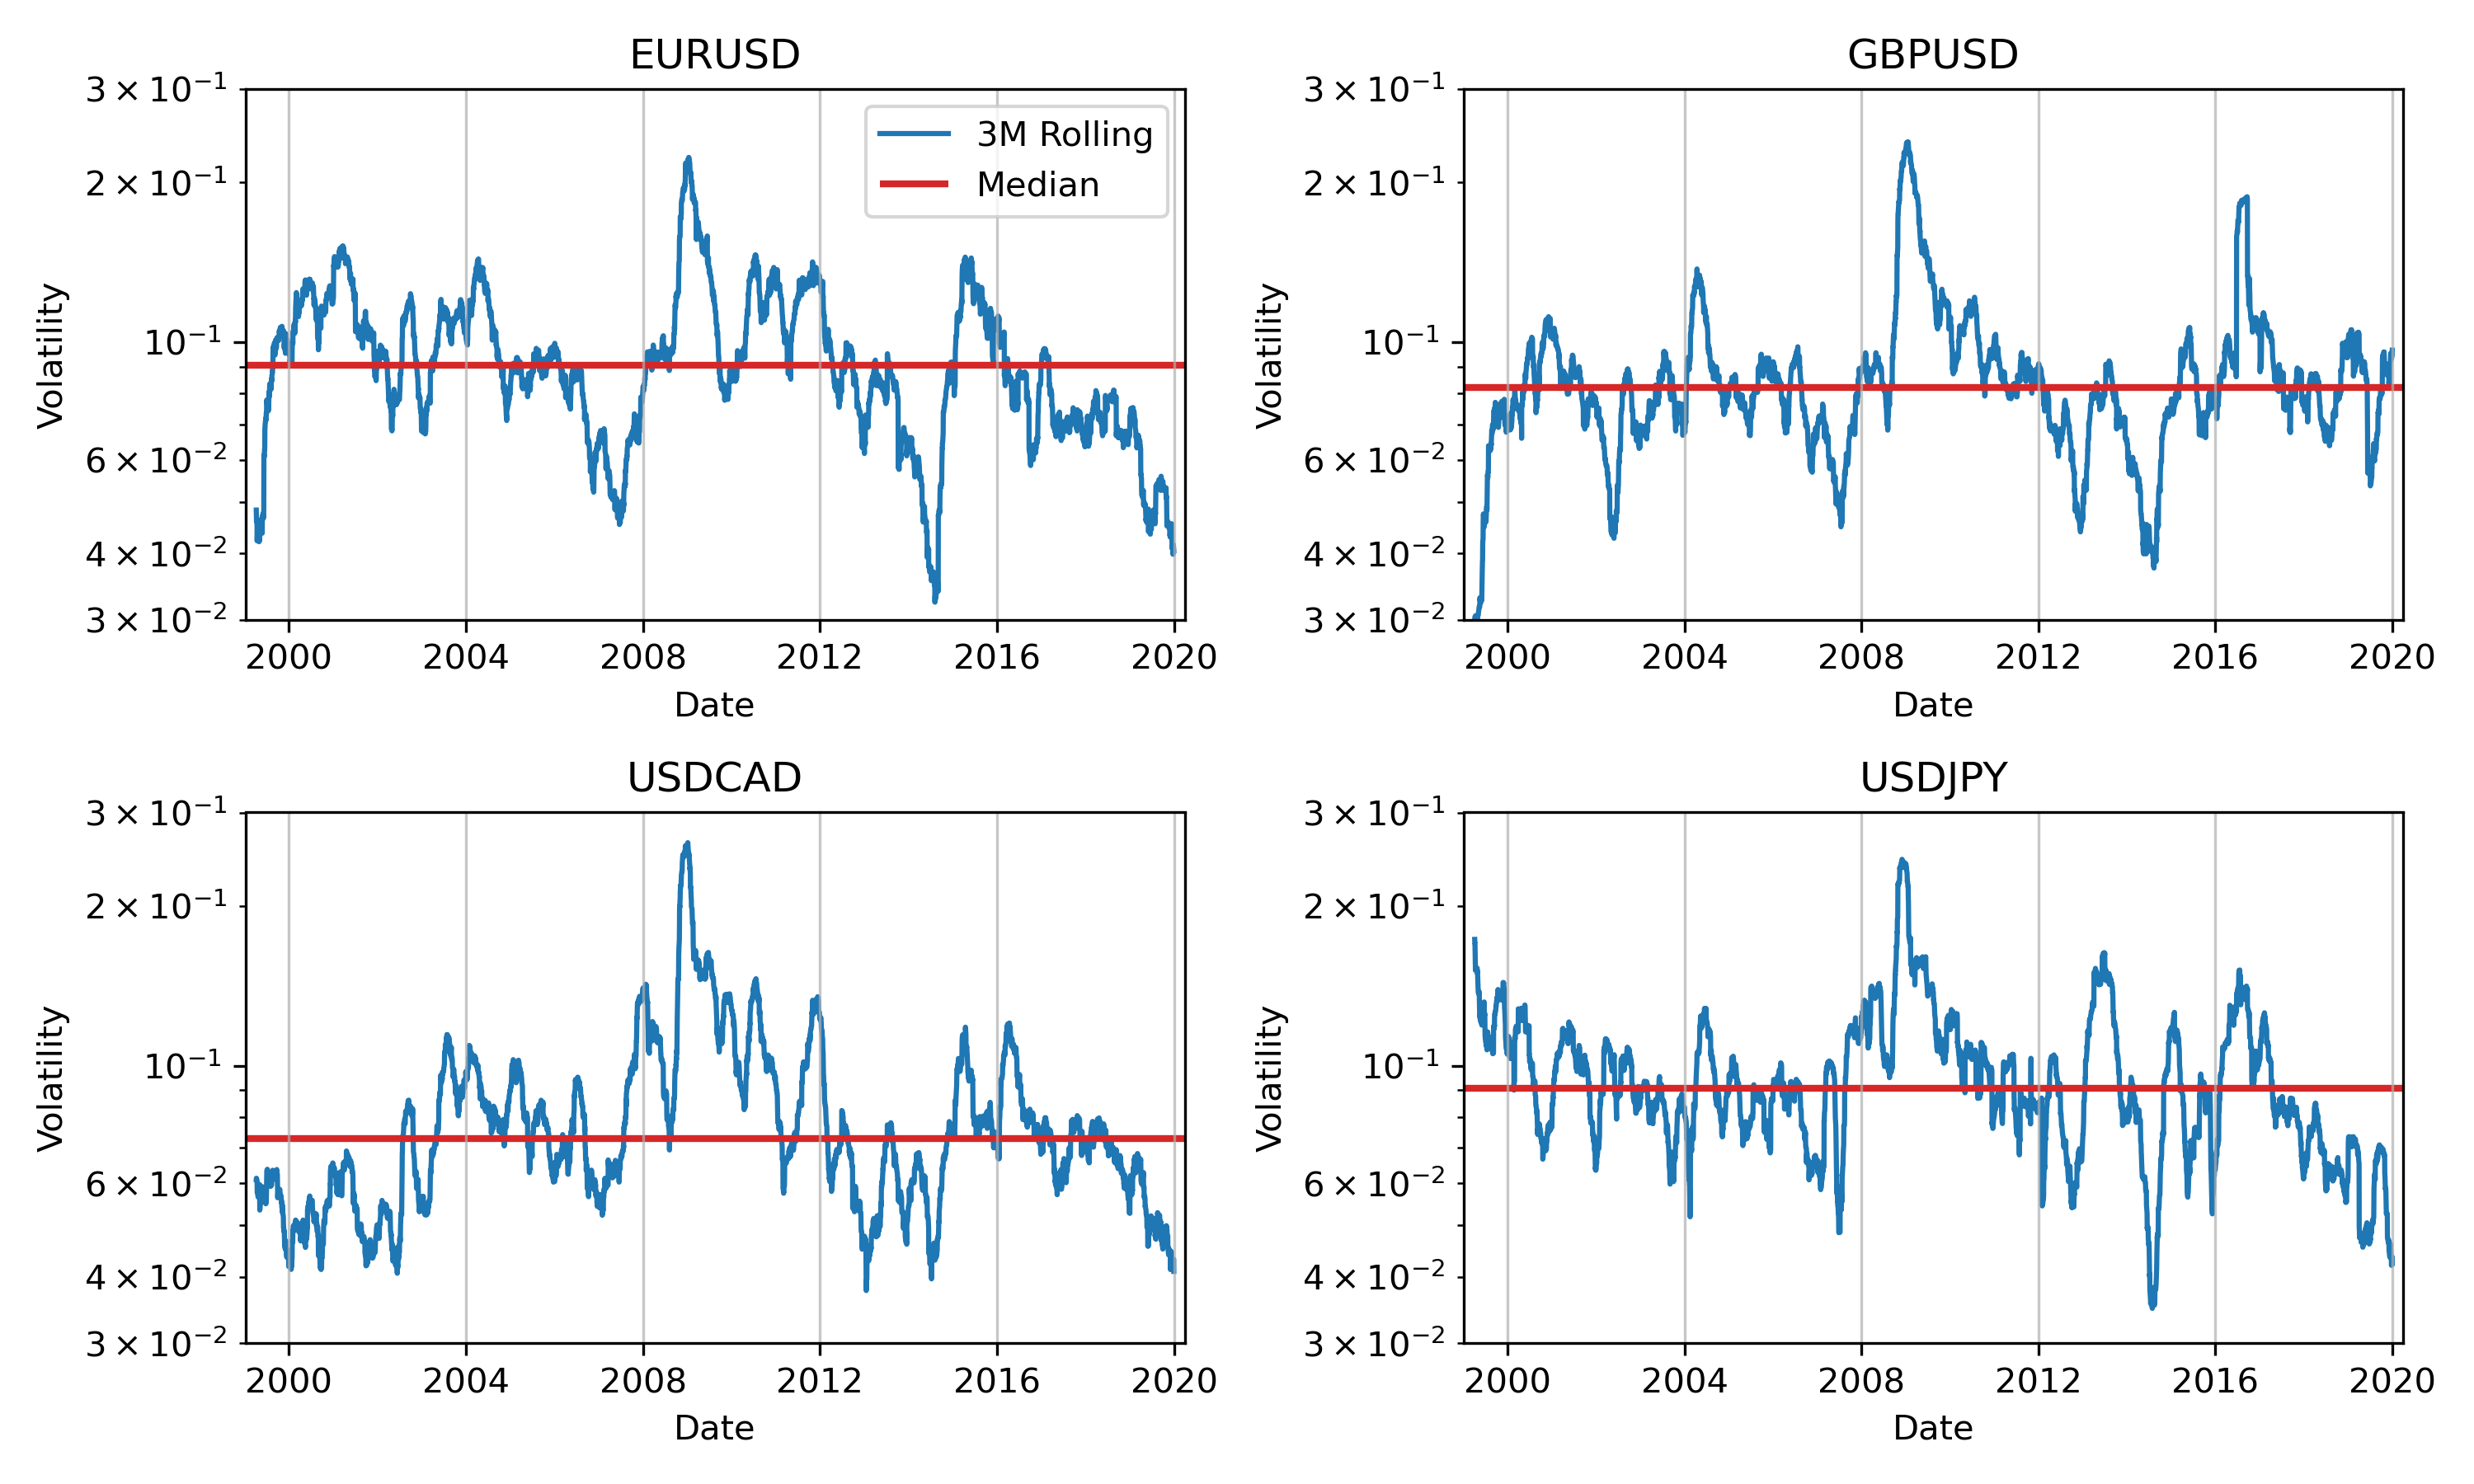
\includegraphics[width=1\linewidth]{data_analysis/rolling_volatility.png}
    \end{center}
    \caption{3-month rolling volatility of the log returns for major currency pairs from 1999-01-01 through 2019-12-31.}
    \label{fig:rolling_volatility}
\end{figure}
